\scanpage{43}
\mspage{17}

On considère que cette donnée équivaut à celle d'une
suite d'inclusions de drapeaux
\[
 d_1\subset d_2\cdots\subset d_p\subset d_{p+1}=d'
 \qquad(p=\operatorname{long}.d')
\]
dont chacun est un segment initial strict de
le \deleted{\unsure{précédent}}\inserted{suivant}.
Ceci donne donc \deleted{des filt} une
suite de projections
\[
 \Sigma_{d'}=\Sigma_{d_{\unsure{p+1|p-1}}}\unsure{-|\longrightarrow}\Sigma_{d_p}
 \unsure{-|\longrightarrow}\cdots\unsure{-|\longrightarrow}\Sigma_{d_2}
 \unsure{-|\longrightarrow}\Sigma_{d_1}
\]
dont on considère le mapping-cône simultané
qu'on désigne par
\[
 C_\Sigma(d_1,d_2,\ldots,
 \underset{\substack{\Vert\\d'}}{d_{\unsure{p+1|p-1}}})
\]
ou aussi par \(\unsure{\mathbb C|C}_{\Sigma,d,d'}\).
On veut déterminer les
morphismes \inserted{\unsure{entre eux}} de transition naturels entre
\[
 C_{\Sigma,d,d'}.
\]

\margin{NB \(d\) est l'ens des
éléments maximaux
des \(d_1,\ldots,d_p\)}

\margin{On reviendra sur cette
\uline{construction} \uline{plus tard}.
Elle n'est pas tellement
utile finalement \(\cdots\)}

\uline{10.} Reprenons la description \unsure{Ab ovo|ab ovo}
(dans le cas \(\mathcal M=(\mathrm{Top})\), pour fixer les idées
--- c'était le contexte adopté au début de ces notes).

\deleted{On}
On a un espace topologique
\figure{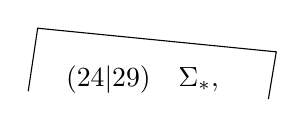
\begin{tikzpicture}[baseline]
 \node at (1.45,0) {\((\unsure{24|29})\quad\Sigma_*,\)};
 \draw (0,-0.15) -- (0.12,0.65) -- (3.15,0.35) -- (3.05,-0.25);
\end{tikzpicture}}
muni d'une relation d'ordre
\[
 \Sigma_{**}\subset\Sigma_*\times\Sigma_*
\]
ayant un graphe fermé, et tel que
\[
 \Sigma_{**}\xrightarrow{\operatorname{pr}_2=\mathrm{but}}\Sigma_*
\]
soit une \deleted{plongement}\inserted{immersion} --- plus

\margin{\textcircled{10}}
\margin{42}
